\documentclass[11pt]{article}
\usepackage{oz,times}

\usepackage{tikz}
\usetikzlibrary{arrows}
\usetikzlibrary{calc}

\title{A Formal Framework for Content-based Retrieval}
\author{Mark d'Inverno and Christophe Rhodes}


\begin{document}
\maketitle


%%\begin{gendef}[X]
%%	concat : (\seq (\seq X)) \fun (\seq X)
%%\where 
%%	\forall xs : \seq X; xss : \seq (\seq X) @ \\
%%\t2		concat~ ((\langle xs \rangle) \cat xss) = xs \cat
%%(concat~xss)  
%%\end{gendef}

%% \begin{gendef}[X]
%%	nfront :  \nat \fun (\seq X)  \fun \seq (\seq X) \\
%% \where 
%%	\forall  n : \nat ; xs : \seq X @ \\
%%		n > \# xs \implies nfront ~n~xs = \langle \rangle  \land \\
%%		n \leq \# xs \implies nfront~n~xs =   \\ 
%%		\t2 (\langle 	(0 \upto n-1) \dres xs    \rangle)    \cat (nfront~n~(tail~xs))
%% \end{gendef}

\section{The System Instance}

\newcommand{\mylet}{\methrel{\sf Let}}
\newcommand{\FV}{\mathrel{~FV}}
\newcommand{\V}{\mathrel{~FV^{d}}}
\newcommand{\U}{\mathrel{~FV^{1}}}
\newcommand{\R}{\mathrel{~R}}

\newcommand{\mylog}{\mathrel{ln}}

\begin{enumerate}

\item \textsf{Track} - original media.

We define the set of all such tracks.

\begin{flushright}
  \begin{tikzpicture}
    \input track.tikz
  \end{tikzpicture}
\end{flushright}

\begin{zed}
[Track]  
\end{zed}

%% \begin{zed}
%%\R == \nat 
%% \end{zed}

%% \begin{axdef}
%% \mylog : \R \fun \R 
%% \end{axdef}




% For every track it is possible to determine the  lenth. 

% \begin{axdef}
%	lenth : Track \fun Time
% \end{axdef} 

% For every track it is possible to determine the  lenth. 

% \begin{axdef}
%	lenth : Track \fun Time
% \end{axdef} 

\item \textsf{Catalogue} - a non-empty list of tracks.

% A catalogue is typically generated for a specific \emph{use case}.  

\begin{flushright}
  \begin{tikzpicture}
    \draw (-3,-3) rectangle (3,3);
    \foreach \y/\xscale in {2/1,1/1.02,0/0.87,-1/0.95} {
      \begin{scope}[yshift=\y cm]
        \begin{scope}[xscale=\xscale]
          \input track.tikz
        \end{scope}
      \end{scope}
    }
    \draw node at (0,-2) {\vdots};
  \end{tikzpicture}
\end{flushright}

\begin{zed}
	Catalogue  == \seq_1 Track 
\end{zed}

\item \textsf{Collection} - a set of catalogues where each track in each catalogue is associated with a unique name.

In a collection, each track has a unique \textsf{TrackName}. We define the injective function $name$ to do this. 

\begin{zed}
	[TrackName]
\end{zed}

\begin{schema}{Collection}
	collection : \power Catalogue 		\\
	tracks : \power Track 			\\
	name : Track \inj TrackName 
\where
	tracks = \{ cat : collection; t : Track | t \in (\ran cat) @ t \}  \\
	\dom name = tracks
\end{schema}




\item \textsf{Time} - the set of non-negative reals. 


\begin{zed}
	Time == \R
\end{zed}





\item \textsf{Interval} - defined as a continuous set of real numbers,  represented as an ordered pair of reals with the second of the pair strictly greater.  

\begin{flushright}
  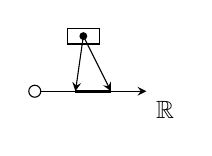
\begin{tikzpicture}[>=stealth]
    \draw (0,0.8) rectangle (0.4,1);
    \fill (0.2,0.9) ellipse (0.05);
    \draw[->] (0.2,0.9) -- (0.1,0.2);
    \draw[->] (0.2,0.9) -- (0.55,0.2);
    \draw[very thick] (0.1,0.2) -- (0.55,0.2);
    \draw[o->] (-0.5,0.2) -- (1,0.2) node[anchor=north west] {\small $\mathbb{R}$};
  \end{tikzpicture}
\end{flushright}

\begin{zed}
	Interval == \{ t_1, t_2 : Time | t_2 > t_1 @ (t_1, t_2) \} 
\end{zed}

\item \textsf{Interval Index} - list of intervals such that the start of each successive interval strictly increases.  Intervals may be overlapping. 

The predicate below states that for any consecutive intervals in an interval index $i_j$ and $i_{j+1}$, that $i_j$ starts before $i_{j+1}$.

\begin{flushright}
  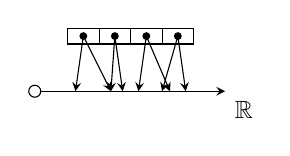
\begin{tikzpicture}[>=stealth]
    \draw (0,0.8) rectangle (1.6,1);
    \draw (0.4,0.8) -- (0.4,1);
    \draw (0.8,0.8) -- (0.8,1);
    \draw (1.2,0.8) -- (1.2,1);
    \fill (0.2,0.9) ellipse (0.05);
    \fill (0.6,0.9) ellipse (0.05);
    \fill (1.0,0.9) ellipse (0.05);
    \fill (1.4,0.9) ellipse (0.05);
    \draw[->] (0.2,0.9) -- (0.1,0.2);
    \draw[->] (0.2,0.9) -- (0.55,0.2);
    \draw[->] (0.6,0.9) -- (0.55,0.2);
    \draw[->] (0.6,0.9) -- (0.7,0.2);
    \draw[->] (1.0,0.9) -- (0.9,0.2);
    \draw[->] (1.0,0.9) -- (1.3,0.2);
    \draw[->] (1.4,0.9) -- (1.2,0.2);
    \draw[->] (1.4,0.9) -- (1.5,0.2);
    \draw[o->] (-0.5,0.2) -- (2,0.2) node[anchor=north west] {\small $\mathbb{R}$};
  \end{tikzpicture}
\end{flushright}

\begin{zed}
	IntervalIndex == \iseq Interval   \\ \\ \\
\end{zed}

\[ 	\forall i : IntervalIndex; i_j, i_{j+1} : Interval @  \\
\t3	\langle i_j, i_{j+1} \rangle \inseq i \implies first~ i_j \leq first ~ i_{j+1}
	\]

\item \textsf{Continuous Interval Index - CII} - there are no consecutive intervals $i_j$ and $i_{j+1}$ in the index where the second element of $i_j$ is strictly less than the first element of $i_{j+1}$.  

\begin{flushright}
  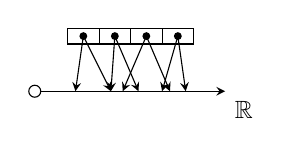
\begin{tikzpicture}[>=stealth]
    \draw (0,0.8) rectangle (1.6,1);
    \draw (0.4,0.8) -- (0.4,1);
    \draw (0.8,0.8) -- (0.8,1);
    \draw (1.2,0.8) -- (1.2,1);
    \fill (0.2,0.9) ellipse (0.05);
    \fill (0.6,0.9) ellipse (0.05);
    \fill (1.0,0.9) ellipse (0.05);
    \fill (1.4,0.9) ellipse (0.05);
    \draw[->] (0.2,0.9) -- (0.1,0.2);
    \draw[->] (0.2,0.9) -- (0.55,0.2);
    \draw[->] (0.6,0.9) -- (0.55,0.2);
    \draw[->] (0.6,0.9) -- (0.9,0.2);
    \draw[->] (1.0,0.9) -- (0.7,0.2);
    \draw[->] (1.0,0.9) -- (1.3,0.2);
    \draw[->] (1.4,0.9) -- (1.2,0.2);
    \draw[->] (1.4,0.9) -- (1.5,0.2);
    \draw[o->] (-0.5,0.2) -- (2,0.2) node[anchor=north west] {\small $\mathbb{R}$};
  \end{tikzpicture}
\end{flushright}

%% 	\begin{zed}
%% ContinuousIntervalIndex == IntervalIndex
%% \end{zed}

%%unchecked
\begin{zed}
	ContinuousIntervalIndex == \\
	\t1 \{ ii : IntervalIndex;  i_j, 
	i_{j+1}: Interval  |   \\
	\t3 \langle i_j, i_{j+1} \rangle \inseq ii \implies  second ~ i_j \geq first ~ i_{j+1}@ ii \}
\end{zed}


\item A \textsf{Duration} is an amount of time. 

\begin{zed}
	Duration == Time
\end{zed}

\item The \textsf{Track Duration} is the duration of a track. It is the difference between the \emph{end} time and \emph{start} time of the track. 

\begin{axdef}
	trackduration : Track \fun Duration 
\end{axdef}

\item \textsf{Interval Duration} is the duration of an interval. It is calculated by subtracting the first element of the interval from the second element. 

\begin{axdef}
	intervalduration : Interval \fun Duration 
\where
	\forall i : Interval @ intervalduration ~ i = second ~ i - first ~ i 
\end{axdef}


\item \textsf{Index Duration} is the duration of a Continuous Interval Index. It is calculated by subtracting the first element of the first interval from the second element of the last interval. 


\begin{axdef}
	indexduration : ContinuousIntervalIndex \fun Time 
\where
\forall cii : ContinuousIntervalIndex @ \\
\t1		indexduration~cii = second (last~cii) - first (head~cii) 
\end{axdef} 

\item \textsf{Segmenter} - a process which computes an interval index  for any track, represented as a function which maps any track to an interval index.

\begin{flushright}
  \begin{tikzpicture}
    \input interval-index.tikz
    \input segmented-track.tikz
  \end{tikzpicture}
\end{flushright}

\begin{zed}
	Segmenter == Track \fun IntervalIndex  \\
\end{zed}

\item The \textsf{Length} of an interval index is the number of intervals contained within it. 

\begin{axdef}
	length : IntervalIndex \fun \nat 
\where
	\forall ii : IntervalIndex @ length~ii = \# ii
\end{axdef}

% \section{Features}

\item \textsf{Feature Name} - a name describing a feature.

\begin{zed}
	[FeatureName]
\end{zed}

\item \textsf{Dimension} - a natural number.

\begin{zed}
	Dimension ==	 \nat
\end{zed}

\item \textsf{Feature Kind} - a feature name and associated set of parameters. 

\begin{zed}
	[Const, Var]
\end{zed}

We define the binding type as the set of functions between variables and constants. 

\begin{zed}
	Binding == \power (Var \cross Const) 
\end{zed}

Every feature kind has a dimension (not necessarily fixed). 

\begin{schema}{FeatureKind}
	name :  FeatureName \\
	parameters : \power Var \\
	dparameters : \power Var \\
	binding : Binding \\
	ddimension : Binding \pfun \nat  \\ 
	fdimension : Dimension  \\
\where
	dparameters  \subseteq parameters  \\
	\forall b : Binding |  b \in (\dom ddimension) @ dparameters \subseteq  (\dom b) 
\end{schema}

\item A \textsf{Feature} -  sometimes referred to as a Fully Qualified Feature - is  a feature kind with all parameters bound. 

\item \textsf{Feature Dimension} - every feature has a fixed  dimension. 

\begin{schema}{Feature}
	FeatureKind \\
\where
	\dom binding = parameters \\
	fdimension = ddimension~binding
\end{schema}

\item \textsf{Unit Feature} - any feature with a dimension of 1.
	
\begin{schema}{UnitFeature}
	Feature \\
\where
	fdimension = 1
\end{schema}

\item \textsf{Feature Vector} - a non-empty sequence of real numbers.

\begin{zed}
	\FV == \seq_1 \R 
\end{zed}

% DEFINE ALL FEATURE VECTORS HERE 

%% \begin{zed}	
%% \V == \FV \\
%% \U  == \FV 
%% \end{zed}

\newcommand{\Vdsl}{\mathrel{~FV^{d * sl}}}

%% \begin{zed}
%% \Vdsl == \FV
%% \end{zed}

\newcommand{\Vd}{\mathrel{~FV^{d}}}

%% \begin{zed}
%% \Vd == \FV
%% \end{zed}

\newcommand{\Z}{\mathrel{~FV^{1}}}

%% \begin{zed}
%% \Z == \FV
%% \end{zed}

\newcommand{\Vsl}{\mathrel{~FV^{sl}}}

%% \begin{zed}
%% \Vsl == \FV
%% \end{zed}


\item \textsf{Feature Vector Dimension} - the length of a feature vector. 

\begin{axdef}
	dimension : \FV \fun \nat
\where
	\forall fv : \FV @ dimension~fv = \# fv
\end{axdef}

\item \textsf{Unit Vector} - any feature vector with a dimension of 1.

\begin{zed}
	UnitVector == \{ fv : \FV | dimension~fv = 1 \}
\end{zed}

\item \textsf{Extractor} - a  process which computes a feature vector of fixed dimension for any interval of any track, represented formally as a function that takes a track and an interval and returns a feature vector.

\begin{zed}
	Extractor ==  Track \fun Interval \fun \FV 
\end{zed}

\item \textsf{Unit Extractor} - a subclass of Extractor where the feature vector dimension is equal to 1.

\begin{zed}
	UnitExtractor ==  \\
\t1		\{ e : Extractor | \forall t : Track; i : Interval @ dimension (e~t~i) = 1 \}  
\end{zed}

\item \textsf{Bel Unit Extractor} - a subclass of Unit Extractor where the function outputs on the bel scale (between minus infinity and zero). 

\begin{zed}
	BelUnitExtractor ==  UnitExtractor
\end{zed}

\item \textsf{Feature Extractors} - the set of  all extractors associated with a feature.

As this data structure can be updated over time -  by adding and removing new features, and adding and removing extractors for a feature as new ones arise and old ones are not used - we use a schema. The  predicate states that the feature vector dimension computed by an extractor must be equal to the associated feature dimension. Every feature has a unique associated unit feature  and every extractor has a unique associated unit extractor. Once a user defines a feature, and one its associated extractors, the unit feature and extractor are generated automatically.  

\begin{schema}{FeatureExtractors}
	featureextractors : Feature \pfun (\power Extractor) \\
	features : \power Feature \\
	extractors : \power Extractor \\
\where
	\dom featureextractors = features \\
	\bigcup (\ran featureextractors) = extractors \\
	\forall f : Feature ; e :  Extractor ; t : Track; i : Interval \\
	\t1 @ e \in featureextractors(f)  \implies  \\
	\t2 f.fdimension = dimension (e~ t ~ i) \\
\end{schema}

The range of the real contained in the bel unit vector is less than 0. 

\begin{zed}
		\forall t : Track; int : Interval; ux : BelUnitExtractor   @  \\
		\t5 head (ux~t~int)  \leq 0
\end{zed}

\item \textsf{Track Feature Vectors} - given a segmenter and an extractor the  sequence of feature vectors  for each interval of the track 

\begin{flushright}
  \begin{tikzpicture}
    \input track-feature-vectors.tikz
  \end{tikzpicture}
\end{flushright}

The function $extract$ applies an extractor to each interval of a track to return a list of feature vectors. This  requires  the generic function  map, which takes a function and applies it to every element of a list. A definition can be found in the appendix. 

%%\begin{gendef}[X,Y]
%%	map : (X \fun Y) \fun (\seq X) \fun (\seq Y) \\
%%\where 
%%	\forall  f : X \fun Y; x : X; xs,ys : \seq X @ \\
%%\t1		map~f~\langle \rangle = \langle \rangle \land \\
%%\t1 		map~f~(xs \cat ys) = map~f~xs \cat map~f~ys 
%%\end{gendef}

\begin{axdef}
extract : Segmenter \fun Extractor \fun Track \fun \seq \FV
\where
\forall seg : Segmenter; fx : Extractor; t : Track @ \\
\t5  extract~seg~fx~t = map ~ (fx~t) (seg~t)
\end{axdef}  


\item \textsf{Track Unit Vectors} - defined as above but specifically for unit extractors

\begin{flushright}
  \begin{tikzpicture}
    \input interval-index.tikz
    \input segmented-track.tikz
%    \foreach \x in {-2.5,-2,-1.4,-0.5,0,0.8,1.3,1.8} {
%      \begin{scope}[xshift=\x cm,yshift=-0.4 cm]
    \foreach \x in {-1.8,-1.4,...,1.1} {
      \begin{scope}[xshift=\x cm,yshift=1.1 cm]
        \draw (-0.1,0) rectangle (0.1,0.2);
      \end{scope}
    }
    \begin{scope}[yshift=1.1 cm]
      \draw[|-|,>=stealth] (-2.3,0) -- (-2.3,0.2);
      \draw node[anchor=south east] at (-2.4,0.1) {\small $d=1$};
    \end{scope}
  \end{tikzpicture}
\end{flushright}

\item \textsf{Catalogue Feature Vectors}  - a sequence of track feature vectors for each track in the target instance ($catfeatures$)

\item  \textsf{Catalogue Unit Vectors}  - a sequence of track unit vectors for each track in the target instance ($catunits$)

\item \textsf{Instance} - a catalogue, segmenter, feature, extractor, unit  feature, unit extractor, dimension, catalogue feature vectors, 

% \emph{In our usage (see \textsf{Absolute} \and \textsf{Relative} in section \ref{s:refining}), we require certain semantics of the \textsf{Unit Feature} (and so of the values returned by its \textit{Unit Extractors}.  Specifically, the values returned must be interpretable on a logarithmic scale in Bels, with the maximum possible value being the reference threshold at 0B.}

\begin{schema}{Instance} 
	cat : Catalogue 				\\
%	tracks : \power Track 	\\
	seg : Segmenter  			\\ 
	f : Feature 				\\  
	x : Extractor				\\			
	uf : UnitFeature			\\
	ux : UnitExtractor			\\
	d : Dimension \\
	catfeatures  :  \seq ~ (	\seq 	\V) \\
	catunits : \seq ~ (\seq 	\U)  
\where
	d = f.fdimension \\
	catfeatures = map ~ (extract~seg~x) ~ cat \\  
	catunits =  map ~ (extract~seg~ux) ~ cat  \\     
\end{schema}	

\item  \textsf{System Instances}  - the set of System instances.

Note that every instance must contain a catalogue in the music collection but not all catalogues in the collection will be part of an instance. 

\begin{schema}{SystemInstances}
		Collection \\
		instances : \power Instance
\where
		\{ i : instances @ i.cat \} \subseteq collection
\end{schema}
		
\section{Search}

\item \textsf{Search Vectors}

Searching takes place using concatenations of feature vectors to build \emph{search} vectors. For a particular query all search vectors will have a fixed length equal to some multiple (which we will refer to as $sl$) of the dimension of the orignal feature vectors ($d$). 

In the schema below, the function $makesearchvs$ takes a natual number $sl$ and a sequence of feature vectors (associated with a track) to create a sequence of search vectors. The first element of the returned sequence is the concatenation of the first $sl$ feature vectors, the second element is also the concatenation the next $sl$ feature vectors but starting from the second element, and so on until all such sequences are formed.  It should be clear that if the original sequence contains $n$ feature vectors then the output will contain $n-sl+1$ vectors. 

\begin{flushright}
  \begin{tikzpicture}[>=stealth]
    \begin{scope}[xshift=-6 cm]
      \input track-feature-vectors.tikz
      \begin{scope}[yshift=1.1 cm]
        \begin{scope}[yshift=1.1 cm,xshift=-1.8cm]
          \input fv1.tikz
          \draw (-0.1,0) rectangle (0.1,1);
          \draw (-0.1,0.2) -- (0.1,0.2);
          \draw (-0.1,0.4) -- (0.1,0.4);
          \draw (-0.1,0.6) -- (0.1,0.6);
          \draw (-0.1,0.8) -- (0.1,0.8);
        \end{scope}
        \begin{scope}[yshift=2.2 cm,xshift=-1.8cm]
          \input fv2.tikz
          \draw (-0.1,0) rectangle (0.1,1);
          \draw (-0.1,0.2) -- (0.1,0.2);
          \draw (-0.1,0.4) -- (0.1,0.4);
          \draw (-0.1,0.6) -- (0.1,0.6);
          \draw (-0.1,0.8) -- (0.1,0.8);
        \end{scope}
        \draw[->] (-1.4,1) arc(0:90:0.4 and 0.6);
        \draw[->] (-1.0,1) arc(0:90:0.8 and 1.7);
        \draw[->] (-1.0,1) arc(0:90:0.4 and 0.6);
        \draw[->] (-0.6,1) arc(0:90:0.8 and 1.7);
      \end{scope}
    \end{scope}
    \input interval-index.tikz
    \input segmented-track.tikz
%    \foreach \x in {-2.5,-2,-1.4,-0.5,0,0.8,1.3,1.8} {
%      \begin{scope}[xshift=\x cm,yshift=-0.4 cm]
    \foreach \x/\f in {-1.8/fv0,-1.4/fv1,-1.0/fv2,-0.6/fv3,-0.2/fv4,0.2/fv5,0.6/fv6,1.0/fv7} {
      \begin{scope}[yshift=1.1 cm,xshift=\x cm]
        \input \f.tikz
      \end{scope}
    }
    \foreach \x/\f in {-1.8/fv1,-1.4/fv2,-1.0/fv3,-0.6/fv4,-0.2/fv5,0.2/fv6,0.6/fv7} {
      \begin{scope}[yshift=2.1 cm,xshift=\x cm]
        \input \f.tikz
      \end{scope}
    }
    \foreach \x/\f in {-1.8/fv2,-1.4/fv3,-1.0/fv4,-0.6/fv5,-0.2/fv6,0.2/fv7} {
      \begin{scope}[yshift=3.1 cm,xshift=\x cm]
        \input \f.tikz
      \end{scope}
    }
    \foreach \x in {-1.8,-1.4,...,0.3} {
      \begin{scope}[xshift=\x cm,yshift=1.1 cm]
        \draw (-0.1,0) rectangle (0.1,3);
        \foreach \y in {0.2,0.4,...,2.9} {
          \draw (-0.1,\y) -- (0.1,\y);
        }
      \end{scope}
    }
    \begin{scope}[yshift=1.1 cm]
      \draw[<->,>=stealth] (-2.1,0) -- (-2.1,3);
      \draw node[anchor=east] at (-2.3,1.5) {$d \times sl$};
    \end{scope}
    \begin{scope}[yshift=1.1 cm]
      \draw[<->,>=stealth] (-2,3.2) -- (0.4,3.2);
      \draw node at (-0.8,3.6) {$n - sl + 1$};
    \end{scope}
    \begin{scope}[xshift=0.6 cm,yshift=1.1 cm]
      \draw (-0.1,0) rectangle (0.1,2);
      \foreach \y in {0.2,0.4,...,1.9} {
        \draw (-0.1,\y) -- (0.1,\y);
      }
      \draw[dashed] (-0.1,0) -- (-0.3,1);
      \draw[dashed] (-0.1,1) -- (-0.3,2);
      \draw[dashed] (-0.1,2) -- (-0.3,3);
    \end{scope}
    \begin{scope}[xshift=1.0 cm,yshift=1.1 cm]
      \draw (-0.1,0) rectangle (0.1,1);
      \foreach \y in {0.2,0.4,...,0.9} {
        \draw (-0.1,\y) -- (0.1,\y);
      }
      \draw[dashed] (-0.1,0) -- (-0.3,1);
      \draw[dashed] (-0.1,1) -- (-0.3,2);
    \end{scope}
    \foreach \x in {-1.4,-1.0,...,0.3} {
      \begin{scope}[xshift=\x cm,yshift=1.1 cm]
        \draw[dashed] (-0.1,0) -- (-0.3,1);
        \draw[dashed] (-0.1,1) -- (-0.3,2);
        \draw[dashed] (-0.1,2) -- (-0.3,3);
      \end{scope}
    }
  \end{tikzpicture}
\end{flushright}

\begin{axdef}
 	makesearchvs : \nat \fun  \seq \Vd \fun \seq \Vdsl
\where 
	\forall xs :  \seq \FV ; sl : \nat   @ \\
\t1 sl > \# xs \implies makesearchvs~sl~xs = \langle \rangle  \land \\
\t1 sl \leq \# xs \implies makesearchvs~sl~xs = \\
\t2 concat (\langle (0 \upto sl-1) \dres xs  \rangle)  \cat  makesearchvs~sl (tail~xs)
\end{axdef}

\subsection{Identifying Source and Target}

A search vector is made from a source (sequence) and used to match against a user-defined target (instance).

\item \textsf{Source} -  a track identified by the user in order to define a search.

\item \textsf{Target} - the instance used to match the source against.

\begin{schema}{IdentifySourceTarget}
	source? : Track \\
	tgt? : Instance \\
	SystemInstances
\where
	source?  \in tracks \\
	tgt? \in instances
\end{schema}	

In addition the user can define the part of the source track to be used in the query. This is known as a sequence.  A user defines the sequence by  specifying the start and end points of the sequence index. (Note that there is an underlying assumption that the segmenter of the target returns a continuous interval index when applied to the source.) 

\item \textsf{Track Part} - a continuous sub-section of a track. 

\begin{zed}
	TrackPart == Track
\end{zed}

\item \textsf{Sequence} - the track part required for the search. 

\item \textsf{Sequence Index} - a continuous interval index that defines the sequence. 

\item \textsf{Sequence Length} - the number of  intervals in the sequence index.

\begin{schema}{IdentifySequence}
	IdentifySourceTarget  \\
	start?, end? :  \nat \\
	seqindex : ContinuousIntervalIndex \\
	sl : \nat \\
	sequence : TrackPart
\where
	start? \in \dom (tgt?.seg (source?)) \\ 
	end? \in \dom (tgt?.seg (source?)) \\ 
	seqindex = (start? \upto end?) \dres (tgt?.seg~source?) \\
	sl = end? - start? \\
\end{schema}

\subsection{Source Search and Feature Vectors}

\item The \textsf{Source Feature Vectors} are the set of feature vectors of the sequence. 

\item The \textsf{Source Unit Vectors} are the set of unit vectors of the sequence. 

\begin{schema}{SourceFeatureVectors}
	IdentifySequence  					\\
	sourcefeatures :  \seq \V   		\\
	sourceunits : \seq \U 			\\
\where
	sourcefeatures =  extract ~tgt?.seg~tgt?.x~sequence \\  
	sourceunits =  extract ~ tgt?.seg~tgt?.ux~sequence  \\  
\end{schema}

\item \textsf{Source Search Vector} - the concatenation of the feature vectors of the source sequence.

\item \textsf{Source Unit Search Vector} - the concatenation of the unit vectors of the source sequence.

\begin{schema}{SourceSearchVectors}
	SourceFeatureVectors 			\\
	sourcesearch : \Vdsl			\\
	sourcesearchunits : \Vsl			\\
\where
	sourcesearch = (head~(makesearchvs~sl~sourcefeatures)) \\
	sourcesearchunits = (head~(makesearchvs~sl~sourcefeatures)) \\
\end{schema}

\subsection{Target Search Vectors}

\item \textsf{Target Search Vectors}

We can define these in exactly the same way as for the source, but as we now have a sequence of sequences of search vectors we have to use the map function to apply the $makesearchveors$ to each list

\begin{schema}{TargetSearchVectors}
	IdentifySourceTarget \\
	IdentifySequence\\
	targetsearchvs :  \seq (\seq \Vdsl) \\  
	targetunitsearchvs :  \seq (\seq \Vsl) \\  
\where
	targetsearchvs =  \\
	\t1 map ~ (makesearchvs ~ sl) ~ tgt?.catfeatures  \\
	targetunitsearchvs =  \\
	\t1 map ~ (makesearchvs ~ sl) ~ tgt?.catfeatures  \\
\end{schema}

\item \textsf{Hopped Search Vectors}

Rather then generating all possible search vectors we may wish to general vectors starting at equally distanced intervals in the interval index of the tracks in an instance.  Re refer to the size of this interval as $hop$. 


\begin{axdef}
 	makehopsearchvs : \nat \fun  \nat \fun \seq \Vd \fun \seq \Vdsl
\where 
	\forall xs :  \seq \FV ; sl : \nat  ; hop  : \nat  @ \\
\t1 sl > \# xs \implies makehopsearchvs~sl~hop~xs = \langle \rangle  \land \\
\t1 sl \leq \# xs \implies makehopsearchvs~sl~hop~xs = \\
\t2 concat (\langle (0 \upto sl-1) \dres xs  \rangle)  \cat  \\
\t2 			makehopsearchvs~sl~hop~ ((0 \upto (hop -1)) \ndres xs)
\end{axdef}

This enables us to define a hop size when generating target search vectors

\begin{schema}{TargetSearchHopVectors}
	hop? : \nat \\
	TargetSearchVectors \\
	targethopsearchvs :  \seq (\seq \Vdsl) \\  
	targethopunitsearchvs :  \seq (\seq \Vsl) \\  
\where
	targethopsearchvs =  \\
	\t1 map ~ (makehopsearchvs ~sl ~ hop?) ~ tgt?.catfeatures  \\
	targethopunitsearchvs =  \\
	\t1 map ~ (makehopsearchvs ~ sl ~ hop?) ~ tgt?.catfeatures  \\
\end{schema}

\end{enumerate}


\section{Distance, Power and Duration}	
	
\subsection{Distance of Source Search Vector from Target Search Vector}

We define the scalar product and distance between vectors of equal dimension. 

\begin{axdef}
	scalarproduct : \V \fun \V \fun \R \\
	distance : \V \fun \V \fun \R \\
\end{axdef}

\begin{zed}
	\forall v_1, v_2 : \V @  distance~v_1~v_2 = 2 - scalarproduct~v_1~v_2		
\end{zed}

Then we can define a variable which maintains a list of all distances between the source search vector and the target search vectors. 

\begin{schema}{Distances}
	distances : \seq (\seq \R)  \\
	SourceSearchVectors \\
	TargetSearchVectors \\
\where
	distances = map (map (distance~sourcesearch)) targetsearchvs
\end{schema}

\subsection{Average `power' of a search feature vector} 

For each Search Feature Vector in the target, we take the associated unit values and take the arithmetic mean. 

\begin{axdef}
	average : \V \fun \R
\end{axdef}

\begin{schema}{Powers}
	targetpowers : \seq (\seq \R) \\
	sourcepower : \R \\
	SourceSearchVectors \\
	TargetSearchVectors \\
\where 
	targetpowers = map~(map ~ average) ~ targetsearchvs\\
	sourcepower = head (map~average ~ sourceunits)
\end{schema}

\subsection{Duration of a search feature vector}

Calculate the duration of the sequence for each search vector. (Made from the concatenation of feature vectors each associated with an interval. Add the intervals together to get the duration of the search vector.)

\begin{schema}{Durations}
	targetdurations : \seq (\seq \R) \\
	sourceduration : \R \\
	TargetSearchVectors  \\
	SourceSearchVectors \\
\end{schema}

\subsection{Compiled Data}

The we have a set of compiled data as follows. 

\begin{schema}{CompiledData}
	Distances \\
	Powers \\
	Durations \\
\end{schema}

\section{Refining a Search}
\label{s:refining}

System will first return the index of the track which gives the smallest distance from the source sequence search vector. Suppose this is at (3,4) in the list of lists. This signifies that the closest match is the 3rd track in the catalogue starting at the 4th interval. There are ways of refining the query. 

\begin{enumerate}

\item \textsf{Key List} -  specify specific tracks within a catalogue to search over. 

\item \textsf{Radius} - reject distances which are greater than a given real number radius. 

\item \textsf{Absolute} - reject any target search vectors where the `power' average is less than a specific absolute value.

\item \textsf{Relative} - reject any target search vectors where the `power' average is not within  + or  - a relative value. 

\item \textsf{Duration Ratio} - remove any search vectors whose total interval (duration) is sufficiently different from the duration of the source. 

\item \textsf{Hop Size} - Rather than making search vectors which start with the first feature vectors and then the second feature vector and so on, make sparser search vectors by starting with fv at 1, then fv at $1 + h$, then fv at $1 + 2h$ and so on where h is the hop size. 

\end{enumerate}

We specify what happens when values are given for any of these parameters. 

First, we specify a single output as signifiying a track, a starting interval, a distance, a power and a duration

\begin{schema}{Output} 
	track : Track \\
	index : \nat \\
	distance : \R \\
	duration : \R \\
	power : \R \\
\end{schema}

The System outputs are a sequence of such outputs ordered according to distance. We define a new variable which specifies the modified output that the user can make. 

\begin{schema}{SystemOutput}
	CompiledData  \\
	output! : \seq Output \\
	modifiedoutput! : \seq Output
\where
	\forall o_1, o_2 : Output @ \langle o_1, o_2 \rangle \inseq output! \\
	\t3 \implies o_1.distance \leq o_2.distance 
\end{schema}

\begin{enumerate}

\item Keylist

\begin{schema}{KeyList}
	SystemOutput \\
	k? : \power Track 
\where
	modifiedoutput! = output! \filter \{ o : Output |  o.track \in k? \} 
\end{schema}	

\item Radius
	
The system removes any elements which have a distance greater than the radius.

\begin{schema}{Radius}
	SystemOutput \\
	r? : \R \\
\where
	modifiedoutput! = \\ 
	\t1 output! \filter \{ o : Output | o.distance \leq r? \}
\end{schema}

\item Absolute

\begin{schema}{Absolute}
	SystemOutput \\
	a? : \R \\
\where
	modifiedoutput! = \\
	\t1 output! \filter \{ o : Output | o.power \geq  a? \} 
\end{schema}	
	
\item Relative

%% \begin{axdef}
%%	abs : \R \fun \R
%% \end{axdef}


\begin{schema}{Relative}
	SystemOutput \\
	rel? : \R \\
\where
	modifiedoutput! = \\
	\t1 output! \filter \{ o : Output | abs (o.power  -  sourcepower) \leq rel?  \} 
\end{schema}	

\item Duration Ratio

%%unchecked
\begin{schema}{DurationRatio}
	SystemOutput \\
	d? : \R \\
\where
	modifiedoutput! = \\
	\t1 output! \filter \{ o : Output | \exp ^ {abs \ln (\frac{o.duration}{sourceduration})} \leq d?  \} 
\end{schema}	

\item Hop Size 

\begin{schema}{Hop}
	hop? : \nat \\
	SystemOutput \\
	TargetSearchHopVectors \\
\end{schema}

\end{enumerate}

\section{Setting Thresholds}

\subsection{For an Instance}

\begin{enumerate}
\item Guess several lengths based on understanding of the instance (beat, bar, phrase, section).   ($sl$) 
\item Generate all sequences of length   ($sl$)  from the tracks in the instance 
\item Select pairs of sequences of length ($sl$) which may or may not be from the same track randomly from the instance, compute distance between these pairs, and repeat a fixed number of times. 
\item Tabulate distances
\item Scary maths
 \item Obtain a global threshold 
 \item Set the radius threshold equal to this  value
 \end{enumerate}

\subsection{For a Source Sequence and a Target Instance (I)}

\begin{enumerate}
\item Take the length of the source sequence ($sl$)
\item Generate all sequences of length   ($sl$)  from the tracks in the instance
\item Select a sequence randomly, calculate the distance form the source sequence, and repeat a fixed number of times. 
\item Tabulate distances
\item Scary maths
 \item Obtain a  threshold for this sequence/instance pair 
 \item Set the radius threshold equal to this  value
 \end{enumerate}

\subsection{For a Source Track and a Target Instance (II)}

\begin{enumerate}
\item Choose a length $sl$ which is less than the track length
\item Generate all sequences of length  ($sl$)  from the tracks in the instance
\item Generate all sequences of length  ($sl$) from the source sequence
\item Select one of these source  sequences randomly and one of the sequences from one of the tracks in the instance randomly, calculate the distance form the source sequence, and repeat a fixed number of times. 
\item Tabulate distances
\item Scary maths
 \item Obtain a threshold for this track/instance pair 
 \item Set the radius threshold equal to this  value
 \end{enumerate}

\appendix
\section{Auxillary Definitions}

\subsection{The function $map$}

This requires need the generic function  map, which takes a function and applies it to every element of a list.

%%unchecked
\begin{gendef}[X,Y]
map : (X \fun Y) \fun (\seq X) \fun (\seq Y) \\
\where 
\forall  f : X \fun Y; x : X; xs,ys : \seq X @ \\
\t1		map~f~\langle \rangle = \langle \rangle \land \\
\t1 		map~f~(xs \cat ys) = map~f~xs \cat map~f~ys 
\end{gendef}


\subsection{The function $concat$}

We can do this by making use of the following generic function that takes a list of lists of lists, and concatenates each of the lists together. 

%%unchecked
\begin{gendef}[X]
 	concat : (\seq (\seq X)) \fun (\seq X)
\where 
	\forall xs : \seq X; xss : \seq (\seq X) @ \\
\t2		concat~ ((\langle xs \rangle) \cat xss) = xs \cat
(concat~xss)  
\end{gendef}

\section{Probabilty of chosing a track} 

The longer the track in a target the more sequences it will contain with the same number of intervals with length ($sl$). Therefore the probability of selecting a track is weighted. Once a track has been selected then a sequence within the track is chosen uniformly. 

%% \begin{axdef}
%%	sum : \power \R \fun \R
%% \end{axdef}

%% \begin{axdef}
%%	pairmax : \R \cross \R \fun \R
%% \end{axdef}

%%unchecked
\begin{schema}{CalculateProbabilities}
	i : Instance \\
	sl : \nat  \\
	allslsequences : \nat \\
	SystemInstances \\
	prob : Track \fun \R  \also
\where
	allslsequences = \\
\t1 		sum \{ t : Track @ pairmax ( 	(length (i.seg~t) - sl + 1), 0 ) \}  \also
 	\forall t : Track @  	prob~t =  \frac{length (i.seg~t) - sl + 1}{ allslsequences}
\end{schema}

This uses a function $subsequences$ which takes a sequence of elements $s$ and a natural number $n$ and returns the number of contiguous sequences of length $n$  and a function $sumseq$ which sums the elements in a list. 

\section{Examples illustrating functions}

\subsection{Track Extract}

Given a segmenter, an extractor, and a track, the function $extract$ returns a list of feature vectors for that track. Each feature vector has equal dimension, and each vector corresponds to the equivalent interval in the interval index. As an example, if the feature vectors have dimension $d$, and if there are $m$ intervals defined by the segmenter, and if we adopt the convention that $\V$ represents a vector of length d, this function would return something with the following form: 

\[    \langle V_{1}^{d}, V_{2}^{d} \dots V_{m}^{d} \rangle \] 

When we apply this function to every track in a catalogue (which is a list of tracks) we simply determine a list of such lists. If there are $n$ tracks in a catalogue then our  data would look something like the following. 

\[ catfeatures = \langle ~~ \langle  V_{11}^{d}, V_{12}^{d} \dots V_{1m_{1}}^{d} \rangle \\
\t3 ~~~				      \langle  V_{21}^{d}, V_{22}^{d} \dots V_{2m_{2}}^{d} \rangle \\
\t3				      \dots \\
\t3				      \dots \\
\t3	~~~			      \langle  V_{n1}^{d}, V_{n2}^{d} \dots V_{nm_{n}}^{d} \rangle
      ~~  \rangle 
				    ~~  \]    
 
The unit vector data has exactly the same structure but with different vectors all of dimension 1. 

\[ catunits = \langle ~~ \langle  V_{11}^{1}, V_{12}^{1} \dots V_{1m_{1}}^{1} \rangle \\
\t4 ~~				      \langle  V_{21}^{1}, V_{22}^{1} \dots V_{2m_{2}}^{1} \rangle \\
\t4				      \dots \\
\t4				      \dots \\
\t4	~~~			      \langle  V_{n1}^{1}, V_{n2}^{1} \dots V_{nm_{n}}^{1} \rangle
      ~~  \rangle 
      				    ~~  \]    

\subsection{Making Search Vectors}

Suppose we had the following feature vectors for a track.

\[ \langle V_{1}^{d},  V_{2}^{d} , V_{3}^{d} \rangle \] 

Also suppose that our sequence length $sl$ had a value of 2 and we applied the function $makesearchvs$. We would then make search vectors as follows. 

\[  \t3 \langle  V_{1}^{d} \cat  V_{2}^{d} , V_{2}^{d} \cat V_{3}^{d}   \rangle  \] 

\end{document}

